\documentclass[12pt, oneside]{altsu-report}
\linespread{1,15}
\title{Название проекта}
\author{А.\,А.~Никто}
\groupnumber{595}
\GradebookNumber{1337}
\supervisor{И.\,А.~Шмаков}
\supervisordegree{ст. преп.}
\ministry{Министерство науки и высшего образования}
\country{Российской Федерации}
\fulluniversityname{ФГБОУ ВО Алтайский государственный университет}
\institute{Институт цифровых технологий, электроники и физики}
\department{Кафедра вычислительной техники и электроники}
\departmentchief{В.\,В.~Пашнев}
\departmentchiefdegree{к.ф.-м.н., доцент}
\shortdepartment{ВТиЭ}
\abstractRU{Цель работы --- изучение и сравнение AVR и ARM микроконтроллеров, а также последующая разработка программного продукта на основе полученных в результате исследовательской работы знаний.

В результате выполнения научно-исследовательской работы было проведено знакомство с архитектурой микроконтроллеров AVR и ARM на примере представителя каждого семейства, знакомство с наборами команд для микроконтроллеров семейств AVR и ARM, а также изучены некоторые аппаратные и программные средства для разработки под AVR и ARM микроконтроллеры.}
\abstractEN{Большой текст на английском!}
\keysRU{AVR, ARM, Arduino, микроконтроллер}
\keysEN{computer simulation, distributed version control}

\date{\the\year}

% Подключение файлов с библиотекой.
\addbibresource{graduate-students.bib}

\begin{document}
\begin{titlepage}
 \begin{center}
    \normalsize
    МИНИСТЕРСТВО НАУКИ И ВЫСШЕГО ОБРАЗОВАНИЯ \\
    РОССИЙСКОЙ ФЕДЕРАЦИИ \\
    ФГБОУ ВО «АЛТАЙСКИЙ ГОСУДАРСТВЕННЫЙ УНИВЕРСИТЕТ»
    \vfill
     
    Институт цифровых технологий, электроники и физики (ИЦТЭФ) \\
    Кафедра вычислительной техники и электроники (ВТиЭ)
    \vfill
     
    \textbf{Изучение и сравнение AVR и ARM микроконтроллеров} \\
    Отчет по научно-исследовательской работе
 \end{center}
\vfill
 
\newlength{\ML}
\settowidth{\ML}{«\underline{\hspace{3cm}}»}
\hfill\begin{minipage}{0.41\textwidth}
  Выполнил: студент 595 гр.\\
  \underline{\hspace{\ML}} А.\,В.~Лаптев \\
  Проверил: ст. преп. кафедры ВТиЭ\\
  \underline{\hspace{\ML}} И.\,А.~Шмаков \\
  «\underline{\hspace{1cm}}» \underline{\hspace{3cm}} 2022 г.
\end{minipage}%
\vfill
 
\begin{center}
  Барнаул, 2022 г.
\end{center}
\end{titlepage}

\setcounter{page}{2}
\makeabstract
\tableofcontents

\chapter*{Введение}
\addcontentsline{toc}{chapter}{Введение}

На сегодняшний день практически у каждого есть какое-либо портативное устройство или другая потребительская электроника. В такой технике приоритетом является низкое энергопотребление в сочетании с относительным быстродействием. Этим требованиям отвечают семейства микроконтроллеров AVR и ARM.

Сейчас встраиваемые системы и портативные устройства --- одна из самых быстрорастущих технологических сфер. И, поэтому, разработка под микроконтроллеры и микропроцессоры этих семейств является актуальной. 

В данной научно-исследовательской работе объектом исследования являются микроконтроллеры семейств AVR и ARM.

Целью работы является изучение и сравнение AVR и ARM микроконтроллеров, а также последующая разработка программного продукта на основе полученных в результате исследовательской работы знаний.

Задачи научно-исследовательской работы:

\begin{enumerate}
    \item Знакомство с архитектурой микроконтроллеров AVR и ARM на примере представителя каждого семейства.
    
    \item Знакомство с наборами команд для микроконтроллеров каждого семейства.
    
    \item Изучение имеющихся аппаратных и программных средств для разработки под AVR и ARM микроконтроллеры.
    
    \item Применение полученных знаний для разработки собственного программного продукта.
    
    \item Разработка собственного программного продукта на выбранной аппаратно-программной платформе.
\end{enumerate}

\chapter{Обзор AVR и ARM}
\section{AVR}
\subsection{Коротко об AVR}

AVR --- семейство восьмибитных микроконтроллеров фирмы Atmel, позднее Mic\-rochip, впервые выпущенные в 1996 г. Они представляют собой мощный инструмент, универсальную основу для создания современных экономичных встраиваемых систем многоцелевого назначения.~\cite{kochegarov_trusov}

Микроконтроллеры AVR имеют гарвардскую архитектуру (программа и данные находятся в разных адресных пространствах) и систему команд, близкую к идеологии RISC. Процессор AVR имеет 32 8-битных регистра общего назначения, объединенных в регистровый файл. В отличие от «идеального» RISC, регистры не абсолютно равноправны:~\cite{wikiRUAVR}

\begin{itemize}
    \item три <<сдвоенных>> 16-битных регистра-указателя X(r26:r27), Y(r28:r29), Z(r30: r31); команды, увеличивающие и уменьшающие 16-битное значение (в тех моделях, где они доступны) с непосредственным операндом, работают только с одной из этих пар;

    \item некоторые команды работают только с регистрами r16...r31; к ним относятся команды, работающие с непосредственным операндом;

    \item команда копирования пары регистров (в тех моделях, где доступна) работает только с соседними регистрами, начинающимися с нечётного (r1:r0, r3:r2, ..., r31:r30);

    \item некоторые варианты команд умножения принимают в качестве аргументов только регистры из диапазона r16...r23;

    \item результат умножения (в моделях, где есть такой модуль) всегда помещается в r0:r1; также только эта пара используется в качестве операндов для команды самопрограммирования, при котором основная программа может изменить часть своего кода (где доступна).
\end{itemize}

Сигналы JTAG (TMS, TDI, TDO и TCK) мультиплексированы на порт ввода-вывода. Режим работы --- JTAG или порт --- задаётся соответствующим битом в регистре fuses. МК AVR поставляются с включённым интерфейсом JTAG.

\subsection{Архитектура}

AVR-микроконтроллеры содержат на кристалле следующие аппаратные средства: 8-разрядное процессорное ядро, память программ, оперативную память данных, энергонезависимую память данных, регистры ввода-вывода, схему прерываний, схему программирования, а также периферийные устройства (рис. 1.1)~\cite{arch_avr_2021}.

\begin{figure}[!ht]
    \centering
    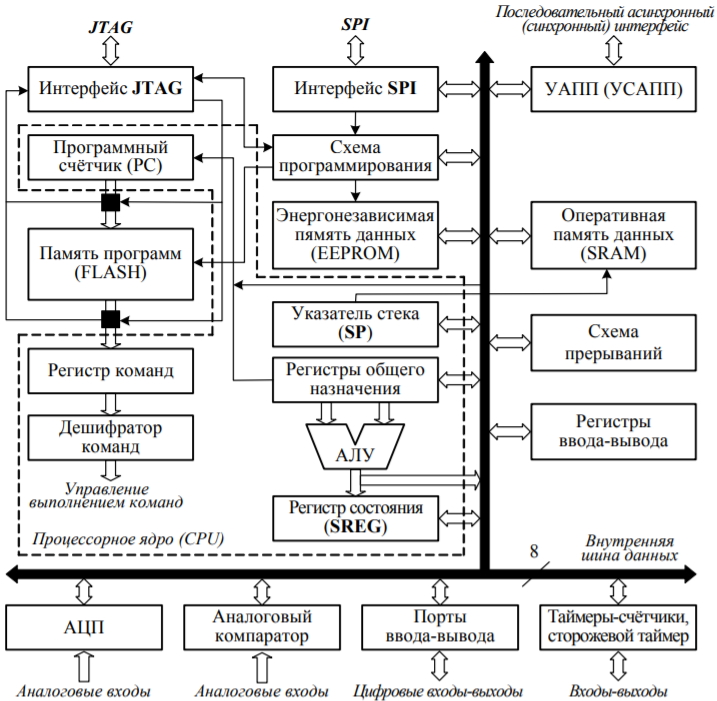
\includegraphics{Architecture_AVR.png}
    \caption{Архитектура микроконтроллеров семейства AVR}
    \label{fig:architecture_arm}
\end{figure}

Процессорное ядро (CPU) AVR-микроконтроллеров содержит арифметико-ло\-гическое устройство (АЛУ), регистры общего назначения (РОН), программный счетчик, указатель стека, регистр состояния, регистр команд, дешифратор команд, схему управления выполнением команд. 

Программный счетчик (PC) содержит адрес следующей выполняемой команды.

Указатель стека (SP) служит для хранения адреса вершины стека.

Регистр состояния (SREG) содержит слово состояния процессора.

АЛУ --- арифметико-логическое устройство, которое синхронно с тактовым сигналом и опираясь на состояние счетчика команд (PC) выбирает из памяти программ (FLASH) очередную команду и производит ее выполнение.~\cite{AVR}

В АЛУ выполняются все вычислительные операции. Операции производятся только над содержимым РОН. На выборку содержимого регистров, выполнение операции и запись результата обратно в РОН затрачивается один машинный такт.

Регистры общего назначения представляют собой 8-разрядные ячейки памяти с быстрым доступом, непосредственно доступные АЛУ. В AVR-микроконтроллерах имеется 32 РОН. Адресное пространство регистров общего назначения размещено в начале оперативной памяти (RAM) но не является ее частью.

FLASH --- память программ, энергонезависимое ПЗУ, выполнено по технологии FLASH. Выполнена в виде последовательности 16-разрядных ячеек, так как большинство команд AVR-микроконтроллера являются 16-разрядными словами. Здесь хранится программа, которая будет исполняться блоком АЛУ микроконтроллера. Флеш-память чипа можно многократно перезаписывать. Данный тип памяти может сохранять записанные в нее данные в течение 40 лет, а количество возможных циклов стирания/записи может достигать 10 000. В зависимости от модели микроконтроллера размер FLASH-памяти может достигать 256 KБ.

EEPROM --- энергонезависимая память данных. В данной памяти можно хранить настройки выполнения программы, собранные данные для статистики работы устройства и другую полезную информацию. Организована как последовательность 8-разрядных ячеек.

Для EEPROM выделено отдельное адресное пространство которое отличается от адресного пространства RAM и FLASH. Память EEPROM микроконтроллера --- очень ценный ресурс, поскольку ее как правило очень мало --- от 0,5 до 4 Кб на чип. Количество перезаписей для данного типа памяти составляет порядка 100 000.

Регистр команд, дешифратор команд и схема управления выполнением команд обеспечивают выборку из памяти программ команды, адрес которой содержится в программном счетчике, ее декодирование, определение способа доступа к указанным в команде аргументам и, собственно, выполнение команды. Для ускорения выполнения команд используется механизм конвейеризации, который заключается в том, что во время исполнения текущей команды программный код следующей выбирается из памяти и декодируется.

Оперативная память данных представляет собой статическое ОЗУ (SRAM) и организована как последовательность 8-разрядных ячеек. Оперативная память данных может быть внутренней (до 32 Кбайт) и внешней (до 64 Кбайт).

Регистры ввода-вывода предназначены для управления процессорным ядром и периферийными устройствами AVR-микроконтроллера.

\subsection{Система команд микроконтроллеров AVR}

Система команд микроконтроллеров AVR весьма развита и насчитывает в различных моделях от 90 до 135 различных инструкций.

Большинство команд занимает только 1 ячейку памяти (16 бит) и выполняется за 1 такт.

Все множество команд микроконтроллеров AVR можно разбить на несколько групп:~\cite{wikiRUAVR}

\begin{itemize}
    \item команды логических операций;

    \item команды арифметических операций и команды сдвига;

    \item команды операции с битами;

    \item команды пересылки данных;

    \item команды передачи управления;

    \item команды управления системой.
\end{itemize}

Управление периферийными устройствами осуществляется через адресное пространство данных. Для удобства существуют <<сокращенные команды>> IN/OUT.~\cite{wikiRUAVR}

\subsection{Семейства и версии микроконтроллеров}

Стандартные семейства микроконтроллеров:

\begin{itemize}
    \item tinyAVR (ATtinyxxx):
    \begin{itemize}
        \item Флеш-память до 16 Кб;
    
        \item SRAM до 512 б;
    
        \item EEPROM до 512 б;
    
        \item Число линий ввода-вывода 4-18 (общее количество выводов 6-32);
    
        \item Ограниченный набор периферийных устройств.
    \end{itemize}
    
    \item megaAVR (ATmegaxxx):
    \begin{itemize}
        \item Флеш-память до 256 Кб;
    
        \item SRAM до 8 Кб;
    
        \item EEPROM до 4 Кб;
    
        \item Число линий ввода-вывода 23-86 (общее количество выводов 28-100);
    
        \item Аппаратный умножитель;
    
        \item Расширенная система команд и периферийных устройств.
    \end{itemize}
    
    \item XMEGA AVR (ATxmegaxxx):
    \begin{itemize}
        \item Флеш-память до 384 Кб;
    
        \item SRAM до 32 Кб;
    
        \item EEPROM до 4 Кб;
    
        \item Четырехканальный DMA-контроллер;
    
        \item Инновационная система обработки событий.
    \end{itemize}
\end{itemize}

Также выделяют семейство микроконтроллеров AVR UC3 --- микроконтроллеры, предназначенные для использования в задачах с высокими требованиями к производительности~\cite{AVR_2016}.

На основе стандартных семейств выпускаются микроконтроллеры, адаптированные под конкретные задачи:

\begin{itemize}
    \item со встроенными интерфейсами USB, CAN, контроллером LCD;

    \item со встроенным радиоприемопередатчиком;

    \item для управления электродвигателями;

    \item для автомобильной электроники;

    \item для осветительной техники. 
\end{itemize}

Кроме указанных выше семейств, ATMEL выпускает 32-разрядные микроконтроллеры семейства AVR32.

Версии контроллеров:~\cite{kochegarov_trusov}

\begin{itemize}
    \item AT(mega/tiny)xxx --- базовая версия.

    \item ATxxxL --- версии контроллеров, работающих на пониженном (Low) напряжении питания (2,7 В).

    \item ATxxxV --- версии контроллеров, работающих на низком напряжении питания (1,8 В).

    \item ATxxxP --- малопотребляющие версии (до 100 нА в режиме Power-down), применена технология picoPower, повыводно и функционально совместимы с предыдущими версиями.

    \item ATxxxA --- уменьшен ток потребления, перекрывается весь диапазон тактовых частот и напряжений питания двух предыдущих версий (также, в некоторых моделях, добавлены новые возможности и новые регистры, но сохранена полная совместимость с предыдущими версиями).
\end{itemize}

\subsection{Программная модель AVR-микроконтроллеров}

Программная модель микропроцессора представляет собой совокупность программно доступных ресурсов. В программную модель микроконтроллеров семейства AVR входят РОН, регистры ввода-вывода, память программ, оперативная память данных и энергонезависимая память данных (рис. 1.2).~\cite{AVR}

\begin{figure}[!ht]
    \centering
    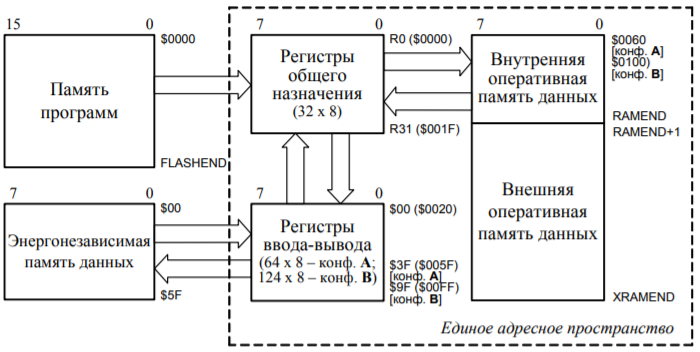
\includegraphics{Program_model_AVR.png}
    \caption{Программная модель AVR-микроконтроллеров}
    \label{fig:program_model}
\end{figure}

РОН (R0...R31) могут использоваться в программе для хранения данных, адресов, констант и другой информации. Шесть старших регистров, как было сказано выше, объединены попарно и составляют три 16-разрядных регистра Х [R27:R26], Y [R29:R28] и Z [R31:R30] (рис. 1.3). 

\begin{figure}[!ht]
    \centering
    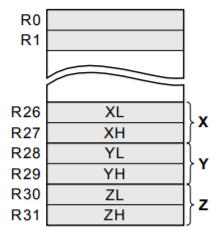
\includegraphics{General_registers.png}
    \caption{Регистры общего назначения}
    \label{fig:gr_avr}
\end{figure}

РОН, регистры ввода-вывода и оперативная память данных образуют единое адресное пространство.

Существует две конфигурации единого адресного пространства памяти AVR-микро\-контроллеров. В конфигурации А младшие 32 адреса (\$0000...\$001F) соответствуют РОН, следующие 64 адреса (\$0020...\$005F) занимают регистры ввода-вывода, внутренняя оперативная память данных начинается с адреса \$0060. В конфигурации В, начиная с адреса \$0060, размещаются 160 дополнительных регистров ввода-вывода; внутренняя оперативная память данных начинается с адреса \$0100. Конфигурация А используется в младших моделях микроконтроллеров и в некоторых старших моделях в режиме совместимости с моделями, снятыми с производства; конфигурация В --- в старших моделях.

В память программ, кроме собственно программы, могут быть записаны постоянные данные, которые не изменяются в процессе работы микроконтроллера (константы, таблицы линеаризации датчиков и т. п.). Выполнение программы при включении питания или после сброса микроконтроллера начинается с команды, находящейся по адресу 0000 памяти программ.

Энергонезависимая память данных предназначена для хранения информации, которая может изменяться непосредственно в процессе работы микропроцессорной системы. Энергонезависимая память данных имеет отдельное адресное пространство и может быть считана и записана программным путем.

Система команд микроконтроллера представляет собой совокупность выполняемых микроконтроллером операций и правил их кодирования в программе. Система команд AVR-микроконтроллеров включает команды арифметических и логических операций, команды ветвления, управляющие последовательностью выполнения программы, команды передачи данных и команды операций с битами. Всего в систему команд входит более 130 инструкций. Младшие модели микроконтроллеров не поддерживают некоторые из них.

\subsection{Периферия}

Микроконтроллеры AVR имеют хорошо развитую периферию.

К периферийным устройствам AVR-микроконтроллера относятся многофункциональные, двунаправленные порты ввода-вывода, таймеры, счетчики, сторожевой таймер, аналоговый компаратор, 10-разрядный 8-канальный АЦП (12-разрядный для XMEGA AVR), универсальный асинхронный (синхронно-асинхронный) приемопередатчик --- УАПП (УСАПП), последовательный периферийный интерфейс (SPI), интерфейс JTAG, устройство сброса по понижению питания, широтно-импульсные модуляторы, датчики температуры и др.~\cite{wikiRUAVR}~\cite{kochegarov_trusov}

Порты ввода-вывода AVR имеют число независимых двунаправленных GPIO линий «вход-выход» от 3 до 86, к которым можно подключить разнообразные датчики, исполняющие устройства и цепи. Каждая линия порта может быть запрограммирована на вход или на выход.

Архитектурная особенность построения портов ввода-вывода у AVR заключается в том, что для каждого физического вывода существует 3 бита контроля/управления, а не 2, как у распространенных 8-разрядных микроконтроллеров (Intel, Microchip, Motorola и т.д.). Это позволяет избежать необходимости иметь копию содержимого порта в памяти для безопасности и повышает скорость работы микроконтроллера при работе с внешними устройствами, особенно в условиях внешних электрических помех.

Система прерываний --- одна из важнейших частей микроконтроллера. Все микроконтроллеры AVR имеют многоуровневую систему прерываний. При возникновении события, вызывающего прерывание, микроконтроллер сохраняет содержимое счетчика команд, прерывает выполнение центральным процессором текущей программы и переходит к выполнению подпрограммы обработки прерывания. После выполнения подпрограммы прерывания осуществляется восстановление предварительно сохраненного счетчика команд и процессор возвращается к выполнению прерванной программы.

Микроконтроллеры AVR имеют в своем составе от 1 до 4 таймеров/счетчиков с разрядностью 8 или 16 бит, которые могут работать и как таймеры от внутреннего источника тактовой частоты, и как счетчики внешних событий~\cite{AVR_2014}.

Их можно использовать для точного формирования временных интервалов, подсчета импульсов на выводах микроконтроллера, формирования последовательности импульсов, тактирования приемопередатчика последовательного канала связи. В режиме ШИМ (PWM) таймер/счетчик может представлять собой широтно-импульсный модулятор и используется для генерирования сигнала с программируемыми частотой и скважностью. Таймеры/счетчики способны вырабатывать запросы прерываний, переключая процессор на их обслуживание по событиям и освобождая его от необходимости периодического опроса состояния таймеров.

Сторожевой таймер предназначен для предотвращения катастрофических последствий от случайных сбоев программы.

Идея использования стоpожевого таймеpа состоит в pегуляpном его сбpасывании под упpавлением пpогpаммы или внешнего воздействия до того, как закончится его выдеpжка вpемени и не пpоизойдет сбpос пpоцессоpа.

Аналоговый компаратор сравнивает напряжения на двух выводах микроконтроллера. Результатом сравнения будет логическое значение, которое может быть прочитано из программы. Выход аналогового компаратора можно включить на прерывание от аналогового компаратора. Пользователь может установить срабатывание прерывания по нарастающему или спадающему фронту или по переключению. Присутствует у всех современных AVR, кроме Mega8515.

Аналого-цифровой преобразователь необходим для получения числового значения напряжения, поданного на его вход. Этот результат сохраняется в регистре данных АЦП. Какой из выводов микроконтроллера будет являться входом АЦП, определяется числом, занесенным в соответствующий регистр. Программируемый коэффициент усиления перед АЦП 1, 10 и 200; в качестве опорного напряжения могут выступать: напряжение питания, внешнее напряжение, или внутреннее некалиброванное опорное напряжение около 2,56 В (для моделей, имеющих минимальное напряжение питания от 2,7 В и выше) либо 1,1 В (с минимальным напряжением питания 1,8 В).

Универсальный асинхронный или универсальный синхронно/асинхронный приемопередатчик (УАПП/УСАПП) --- удобный и простой последовательный интерфейс для организации информационного канала обмена микроконтроллера с внешним миром. Способен работать в дуплексном режиме (одновременная передача и прием данных).

Последовательный периферийный трехпроводный интерфейс (SPI) предназначен для организации обмена данными между двумя устройствами. С его помощью может осуществляться обмен данными между микроконтроллером и различными устройствами, такими, как цифровые потенциометры, ЦАП/АЦП, FLASH ПЗУ и др. С помощью этого интерфейса удобно производить обмен данными между несколькими микроконтроллерами AVR. Кроме того, через интерфейс SPI может осуществляться программирование микроконтроллера.

SPI, зачастую, применяется для обмена данными между несколькими микроконтроллерами со скоростью до нескольких MГц.~\cite{AVR}

Для обмена данными по SPI интерфейсу между двумя устройствами достаточно 3-х проводников:

\begin{itemize}
    \item MOSI (Master Output Slave Input) --- данные от ведущего к ведомому;

    \item MISO (Master Input Slave Output) --- данные от ведомого к ведущему;

    \item CLK (Clock) ---  тактовый сигнал.
\end{itemize}

Устройства с SPI-интерфейсом делятся на два типа: ведущий (Master) и ведомый (Slave). Если к интерфейсу подключено несколько устройств то для обмена данными между ними нужны дополнительные линии связи(проводники) чтобы мастеру можно было выбрать ведомое устройство и сделать запрос к нему.

Также SPI интерфейс используется для внутрисхемного SPI программирования, по этому интерфейсу к микроконтроллеру подключается программатор. 

Двухпроводной последовательный интерфейс (TWI) является полным аналогом базовой версии интерфейса I2C. Этот интерфейс позволяет объединить вместе до 128 различных устройств с помощью двунаправленной шины, состоящей из линии тактового сигнала (SCL) и линии данных (SDA).

В отличие от SPI интерфейса (один мастер и один/несколько ведомых) интерфейс TWI --- двунаправленный, что позволяет организовать между несколькими микроконтроллерами небольшую внутреннюю сеть.

Интерфейс JTAG был разработан группой ведущих специалистов по проблемам тестирования электронных компонентов. В состав интерфейса входят четыре проводника: TDI(Test Data In), TDO(Test Data Out), TCK(Test Clock), TMS (Test Mode Select). Интерфейс JTAG используется для тестирования печатных плат; внутрисхемной отладки, используя блок внутренней отладки (OCD), без использования эмуляторов; программирования микроконтроллеров. Многие микроконтроллеры семейства Mega имеют совместимый интерфейс JTAG или debugWIRE для встроенной отладки. Кроме того, все микроконтроллеры Mega с флэш-памятью емкостью 16 Кбайт и более могут программироваться через интерфейс JTAG.

LCD --- интерфейс для подключения жидкокристаллического индикатора или дисплея.

CAN --- интерфейс для объединения в сеть различных контроллеров и датчиков.

USB --- интерфейс для подключения периферийных устройств.

Тактовый генератор вырабатывает импульсы для синхронизации работы всех узлов микроконтроллера.

Внутренний тактовый генератор AVR может запускаться от нескольких источников опорной частоты:

\begin{itemize}
    \item керамический или кварцевый резонатор (не у всех моделей);

    \item внешний тактовый сигнал;

    \item внутренний RC-генератор (частота 1, 2, 4, 8 МГц, а также, для некоторых моделей ATtiny — 4,8, 6.4, 9.6 МГц и 128 кГц).
\end{itemize}

Минимальная допустимая частота ничем не ограничена (вплоть до пошагового режима). Максимальная рабочая частота определяется конкретным типом микроконтроллера и указывается Atmel в его характеристиках.

Установка источника тактовых импульсов производится с помощью FUSE-битов.

FUSES --- специальные 4 байта данных, которые настраивают некоторые глобальные параметры микроконтроллера в процессе прошивки. После прошивки данные биты нельзя изменить через внутреннюю программу что записана в микроконтроллер.~\cite{AVR}

Данной конфигурацией бит указывается микроконтроллеру:

\begin{itemize}
    \item какой использовать задающий генератор (внешний или внутренний);

    \item делить частоту генератора на коэффициент или нет;

    \item использовать ножку сброса (RESET) для сброса или же как дополнительный пин ввода-вывода;

    \item количество памяти для загрузчика;

    \item другие настройки зависимо от используемого микроконтроллера.
\end{itemize}

Система реального времени (RTC) реализована во всех микроконтроллерах серии Mega. Таймер/счетчик RTC имеет отдельный предделитель, который может быть программным способом подключен или к источнику основной тактовой частоты, или к дополнительному асинхронному источнику опорной частоты (кварцевый резонатор или внешний синхросигнал). Для этой цели зарезервированы два вывода микросхемы. 

Набором периферийных устройств определяются функциональные возможности микроконтроллера.

Обмен информацией между устройствами AVR-микроконтроллера осуществляется посредством внутренней 8-разрядной шины данных.

\subsection{Питание}

AVR функционируют при напряжениях питания от 1,8 до 6,0 В.

AVR могут быть переведены программным путем в один из трех режимов пониженного энергопотребления:

\begin{itemize}
    \item Режим холостого хода --- прекращает работу только процессор и фиксируется содержимое памяти данных, а внутренний генератор синхросигналов, таймеры, система прерываний и сторожевой таймер продолжают функционировать.

    \item Стоповый режим --- сохраняется содержимое регистрового файла, но останавливается внутренний генератор синхросигналов, и, следовательно, останавливаются все функции, пока не поступит сигнал внешнего прерывания или аппаратного сброса.

    \item Экономичный режим --- продолжает работать только генератор таймера, что обеспечивает сохранность временной базы. Все остальные функции отключены.
\end{itemize}

В микроконтроллерах существует специальный режим --- сброс при снижении напряжения питания (BOD). Схема BOD отслеживает напряжение источника питания. Если схема включена, то при снижении питания ниже некоторого значения она переводит микроконтроллер в состояние сброса. Когда напряжение питания вновь увеличится до порогового значения, запускается таймер задержки сброса. После формирования задержки внутренний сигнал сброса снимается и происходит запуск микроконтроллера.~\cite{kochegarov_trusov}

\section{ARM}

\subsection{Коротко об ARM}

Архитектура ARM --- система команд и семейство описаний и готовых топологий 32-битных и 64-битных микропроцессорных/микроконтроллерных ядер, разрабатываемых компанией ARM Limited.

Среди лицензиатов готовых топологий ядер ARM --- компании AMD, Apple, Analog Devices, Atmel, Xilinx, Cirrus Logic, Intel (до 27 июня 2006 года), Marvell, NXP, STMicroelectronics, Samsung, LG, MediaTek, Qualcomm, Sony, Texas Instruments, Nvidia, Freescale, Миландр, ЭЛВИС, HiSilicon, Байкал электроникс.

Значимые семейства: ARM7, ARM9, ARM11 и Cortex.

Многие лицензиаты проектируют собственные топологии ядер на базе системы команд ARM.

Процессоры и микроконтроллеры ARM широко используются в потребительской электронике --- в том числе смартфонах, мобильных телефонах и плеерах, портативных игровых консолях, калькуляторах, умных часах и компьютерных периферийных устройствах, таких, как жесткие диски или маршрутизаторы.

Они имеют низкое энергопотребление, поэтому находят широкое применение во встраиваемых системах и преобладают на рынке мобильных устройств, для которых данный фактор немаловажен.~\cite{wikiRUARM}

\subsection{Архитекутра}

Существует справочное руководство по архитектуре ARM, которое разграничивает все типы интерфейсов, которые поддерживает ARM, так как детали реализации каждого типа процессора могут различаться. Начиная с ARMv7, были определены 3 профиля:

\begin{itemize}
    \item A (application) --- для устройств, требующих высокой производительности (например, смартфоны, планшеты);

    \item R (real time) --- для приложений, работающих в реальном времени;

    \item M (microcontroller) --- для микроконтроллеров, недорогих встраиваемых уст\-ройств.
\end{itemize}

Профили могут поддерживать меньшее количество команд (команды определенного типа).

Микроконтроллеры ARM содержат следующие аппаратные средства: 32-разрядное процессорное ядро, память программ, оперативную память данных, регистры ввода-вывода, а также периферийные устройства (внутренние и внешние) (рис. 1.4)~\cite{Program_model_ARM}.

\begin{figure}[!ht]
    \centering
    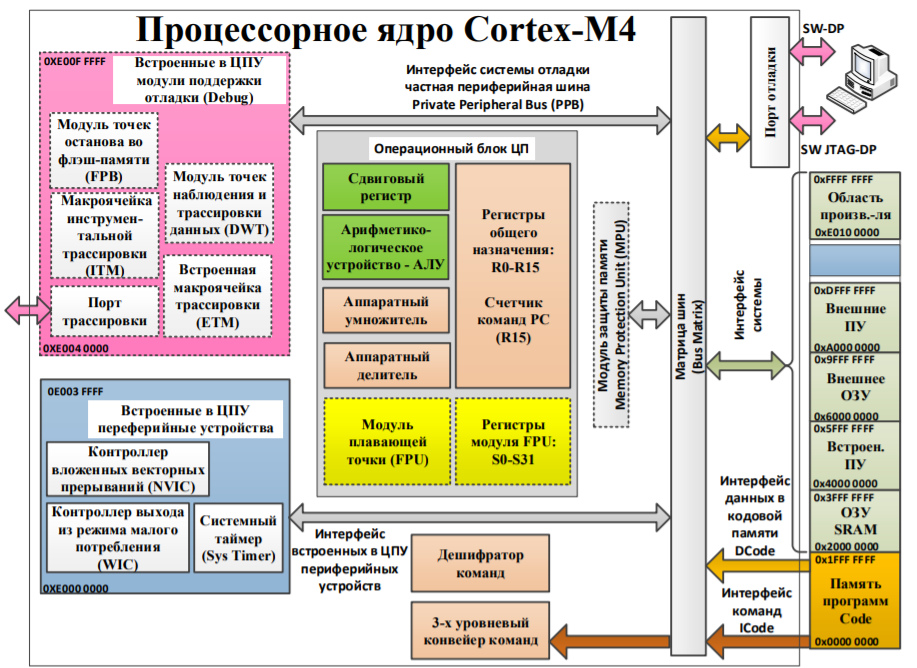
\includegraphics[scale=0.75]{Architecture_ARM.png}
    \caption{Архитектура ARM-микроконтроллера Cortex M4}
    \label{fig:architecture_arm}
\end{figure}

Процессорное ядро ARM-микроконтроллеров содержит в себе операционный блок (состоит из арифметико-логического устройства, аппаратный умножитель, аппаратный делитель, файл регистров общего назначения, сопроцессор для обработки чисел в формате с плавающей точкой (присутствует не во всех моделях), файл регистров сопроцессора (также есть не во всех моделях)), встроенные модули поддержки отладки, встроенные периферийные устройства, дешифратор команд, конвейер команд, модуль защиты памяти.

Арифметико-логическое устройство (АЛУ) --- двухпортовое устройство, которое является ядром операционного блока. Используется для выполнения арифметических, логических и других операций над 32-разрядными операндами. Все операции могут выполняться только над содержимым РОН. Загрузка результата операции также осуществляется в один из РОН.

Имеет дополнительный кольцевой сдвиговый регистр, позволяющий выполнять так называемые <<попутные>> операции сдвига при выполнении большинства обычных операций.

Аппаратный умножитель --- устройство,которое служит для перемножения 32-разрядных чисел в формате с фиксированной точкой с поддержкой операций умножения-накопления, а также с возможностью получения 64-битного результата.

Аппаратный делитель --- устройство, которое служит для деления 32-разрядных чисел со знаком или без знака.

Регистры общего назначения представляют собой 32-разрядные ячейки памяти с быстрым доступом, непосредственно доступные АЛУ. В ARM-микроконтроллерах имеется 16 РОН.

Модуль аппаратной поддержки вычислений в формате с плавающей точкой (FPU) выполняет функцию сопроцессора и обеспечивает:

\begin{itemize}
    \item Обработку операндов, расположенных в 32-разрядных регистрах модуля плавающей точки, которые представляют собой дополнительное сверхоперативное ОЗУ модуля FPU (операнды для обработки могут располагаться только в этом регистровом файле);

    \item Операции обработки 32-разрядных чисел с плавающей точкой однократной точности: преобразования форматов, сложения, вычитания, сравнения, умножения, умножения с накоплением, деления, извлечения квадратного корня;

    \item Операции обычного последовательного умножения с накоплением и одновременного умножения с накоплением повышенной точности;

    \item Расширение диапазона чисел с плавающей точкой однократной точности за счет поддержки операций с денормализованными числами и всех режимов округления.

    \item Извлечение и выполнение команд обработки чисел с плавающей точкой на трехстадийном конвейере с независимой работой стадий конвейера.

    \item Выполнение большинства команд сопроцессора за один такт.
\end{itemize}

В микроконтроллерах ARM используются модули отладки, которые реализованы в архитектуре процессорного ядра.

С их помощью поддерживаются:

\begin{enumerate}
    \item Доступ в режиме отладки ко всей памяти системы и регистрам процессора, включая доступ к регистрам периферийных устройств;

    \item Установка в отлаживаемой программе точек останова, при достижении которых выполнение программы приостанавливается и управление передается отладчику;

    \item Установка точек наблюдения, при достижении которых значения переменных сохраняются для последующего анализа;
    
    \item Трассировка программы, когда она выполняется либо в пошаговом режиме, либо от одной точки останова до другой с возможностью контроля значений переменных;

    \item Профилирование программы. Оценка быстродействия (времени выполнения) всей программы или отдельных ее фрагментов (подпрограмм), частоты обращения к подпрограммам с целью последующей оптимизации наиболее часто используемых фрагментов кода или определения вообще не используемых участков кода;

    \item Вывод отладочной информации на дисплей системы верхнего уровня (компьютер), используемый для отладки;

    \item Сопряжение с анализаторами данных в порту трассировки (TPA);

    \item Доступ к встроенным в процессор отладочным устройствам через два внешних интерфейса, к которым подключаются компьютерные системы отладки верхнего уровня:

    \begin{itemize}
        \item Последовательный отладочный JTAG-порт (SWJDP), являющийся стандартом для производителей отладочного оборудования и микроконтроллеров;
    
        \item Последовательный отладочный порт (SW-DP), широко используемый производителями ARM-процессоров и микроконтроллеров;
    \end{itemize}
\end{enumerate}

В конкретном микроконтроллере может быть либо один из этих интерфейсов, либо оба для сопряжения со средствами отладки разных производителей.

Часто JTAG-порт является универсальным и совмещается с SW-DP-портом.

Функцию дешифрации команды, выполняет дешифратор команд. Дешифратор команд по коду операции запускает соответствующий данной команде дискретный управляющий автомат, задающий последовательность микроопераций, приводящих к выполнению команды. Перед декодированием команды происходит ее загрузка из памяти на 3-х уровневый конвейер команд и команда находится на конвейере до тех пор, пока не поступит на выполнение в операционный блок процессора.

Опциональный модуль защиты памяти (MPU), предназначен для защиты определенных областей памяти от случайного или несанкционированного доступа. Используется в основном в достаточно сложных системах, как правило, имеющих операционную систему реального времени. Области памяти, которые использует программное обеспечение верхнего уровня, могут быть заблокированы для доступа со стороны обычных пользовательских программ, что повышает надежность работы всей системы.

Память программ --- ПЗУ, выполнено по технологии FLASH. Выполнена в виде последовательности 32-разрядных ячеек. Здесь хранится программа, которая будет исполняться блоком АЛУ микроконтроллера. Флеш-память чипа можно многократно перезаписывать.

Оперативная память данных представляет собой статическое ОЗУ (SRAM) и организована как последовательность 32-разрядных ячеек. Оперативная память данных может быть внутренней и внешней.

Среди внутренних периферийных устройств интегрированных в ЦП выделяют:

\begin{itemize}
    \item Контроллер вложенных векторных прерываний (NVIC).

    \item Системный таймер (Sys Timer).

    \item Контроллер выхода из режима малого потребления энергии (WIC).
\end{itemize}

Интеграция такой периферии непосредственно в ЦП позволяет предельно минимизировать затраты времени на обращение к этим устройствам, в том числе, время реакции на прерывания, что является очень важным для систем управления реального времени.

Процессор может находиться в одном из следующих операционных режимов:

\begin{itemize}
    \item User mode --- обычный режим выполнения программ. В этом режиме выполняется большинство программ.

    \item Handler mode --- режим, в который переходит процессор при возникновении исключения.
\end{itemize}

Переключение режима процессора происходит при возникновении соответствующего исключения или же модификацией регистра статуса.

ARM действует на основе RISC-команд, которые содержат готовый набор простейших элементов.~\cite{ARM}

Архитектура ARM обладает следующими особенностями RISC:~\cite{wikiRUARM}

\begin{itemize}
    \item Архитектура загрузки/хранения;

    \item Нет поддержки нелинейного доступа к памяти (поддерживается в процессорах ARMv6, за некоторыми исключениями, и полностью в ARMv7 и более поздних);

    \item Равномерный 16х32-битный регистровый файл;

    \item Фиксированная длина команд (32 бита) для упрощения декодирования за счет снижения плотности кода. Позднее режим Thumb повысил плотность кода.

    \item Одноцикловое исполнение.
\end{itemize}

Чтобы компенсировать простой дизайн, в сравнении с современными процессорами были использованы некоторые особенности дизайна:

\begin{itemize}
    \item Арифметические инструкции заменяют условные коды, только когда это необходимо;

    \item 32-битное многорегистровое циклическое сдвиговое устройство, которое может быть использовано без потерь производительности в большинстве арифметических инструкций и адресных расчетов.

    \item Мощные индексированные адресные режимы;

    \item Регистр ссылок для быстрого вызова функций листьев;

    \item Простые, но быстрые, с двумя уровнями приоритетов подсистемы прерываний с включенными банками регистров.
\end{itemize}

Архитектура предоставляет способ расширения набора команд, используя сопроцессоры.

В машинах на основе ARM периферийные устройства обычно подсоединяются к процессору путём сопоставления их физических регистров в памяти ARM или в памяти сопроцессора, или путём присоединения к шинам, которые, в свою очередь, подсоединяются к процессору.

\subsection{Наборы команд микроконтроллеров ARM}

В архитектуре ARM, на сегодняшний день, существует несколько наборов команд: ARM, Thumb, Thumb-2, Jazelle, A64.

Набор команд ARM представляет из себя базовый набор 32-битных команд.

Набор команд Thumb --- альтернативный набор 16-разрядных команд, который использовался для улучшения плотности кода.

Набор команд Thumb-2 расширяет набор 16-разрядных команд Thumb дополнительными 32-разрядными, чтобы задать набору команд дополнительную ширину. Цель Thumb-2 --- достичь плотности кода, как у Thumb, и производительности, как у набора команд ARM на 32 битах. В ARMv7 эта цель была достигнута.

Thumb-2 расширяет как команды ARM, так и команды Thumb ещё большим количеством команд, включая управление битовым полем, табличное ветвление, условное исполнение.

Jazelle --- это технология, которая позволяет байткоду Java исполняться прямо в архитектуре ARM в качестве 3-го состояния исполнения (и набора команд) наряду с обычными командами ARM и режимом Thumb.

A64 --- 64-битный набор команд, появившийся с приходом версии архитектуры ARMv8.

Как видно из схемы, микроконтроллеры ARM семейства Cortex M из всех перечисленных наборов команд поддерживают лишь наиболее универсальный Thumb-2. Помимо этого у этих микроконтроллеров нет поддержки сопроцессоров VFP и SIMD (NEON) (рис. 1.5).

\begin{figure}[!ht]
    \centering
    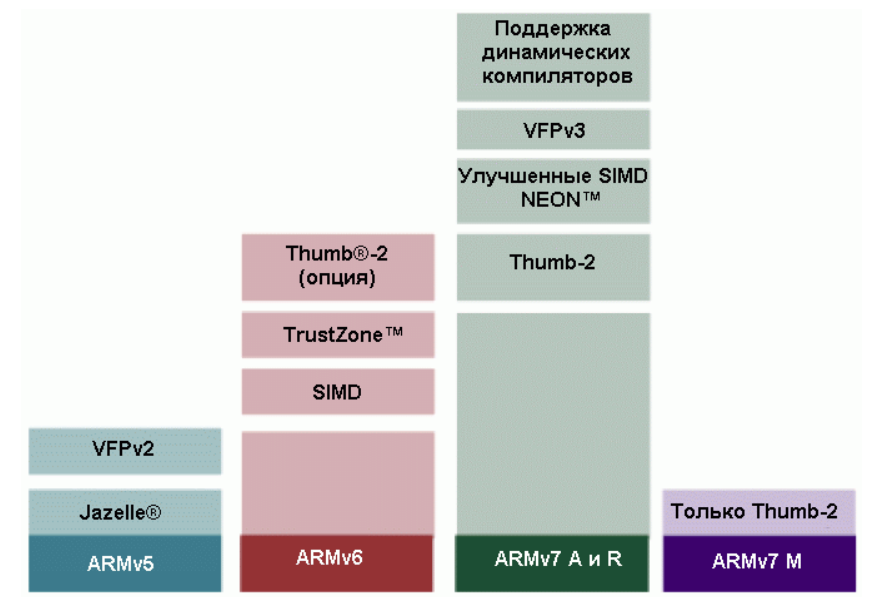
\includegraphics[scale=0.75]{Thumb-2.png}
    \caption{Поддержка наборов команд разными версиями архитектуры ARM}
    \label{fig:thumb-2}
\end{figure}

\subsection{Семейства и версии микроконтроллеров}

Как было описано выше, в ARM были определены 3 профиля процессоров:

\begin{itemize}
    \item A (application) --- для устройств, требующих высокой производительности (например, смартфоны, планшеты);

    \item R (real time) --- для приложений, работающих в реальном времени;

    \item M (microcontroller) --- для микроконтроллеров, недорогих встраиваемых уст\-ройств.
\end{itemize}

Среди микроконтроллеров в настоящее время значимым являются семейство Cortex M~\cite{wikiRUARM}.

Cortex M --- новое семейство микроконтроллеров, призванное занять новую для ARM нишу встраиваемых решений низкой производительности. В семействе присутствуют четыре значимых ядра:

\begin{itemize}
    \item Cortex-M0, Cortex-M0+ (более энергоэффективное) и Cortex-M1 (оптимизировано для применения в ПЛИС) с архитектурой ARMv6-M;

    \item Cortex-M3 с архитектурой ARMv7-M;

    \item Cortex-M4 (добавлены SIMD-инструкции, опционально FPU) и Cortex-M7 (FPU с поддержкой чисел одинарной и двойной точности) с архитектурой ARMv7E-M;

    \item Cortex-M23 и Cortex-M33 с архитектурой ARMv8-M.
\end{itemize}

\subsection{Программная модель ARM-микроконтроллеров}

Программная модель микроконтроллера ARM состоит из следующих блоков: регистры общего назначения, регистр управления Control, регистр команд, Сдвиговый регистр, регистр статуса программы, память программ (ROM), память данных (RAM), а также регистров модуля поддержки вычислений с плавающей точкой (FPU) и регистра статуса и управления FPU (последние два блока встречаются не во всех моделях микроконтроллеров).

Регистры общего назначения (РОН), которые также называют регистровым окружением центрального процессора, необходимы, в первую очередь, для работы операционного блока процессора (включает в себя арифметико-логическое устройство (АЛУ), аппаратный умножитель, аппаратный делитель, сдвиговый регистр), поскольку этот блок оптимизирован для работы только с регистровым окружением. При этом последние 3 регистра имеют специальные функции (рис. 1.6).

Регистр r15 служит счетчиком команд (PC) и содержит адрес следующей выполняемой команды.

Регистр r14 --- регистр связи (LR). Содержит адрес возврата в основную программу после команды вызова подпрограммы.

Регистр r13 –-- регистр-указатель стека (SP). Состоит из двух регистров:

\begin{itemize}
    \item PSP –-- указатель стека процесса пользователя (программ нижнего уровня);

    \item MSP –-- указатель стека обработчиков исключений и программ верхнего уровня.
\end{itemize}

Перед выполнением любой операции в регистры-источники должны быть предварительно загружены исходные данные --- операнды. Результат операции также сохраняется в одном из <<регистров окружения>> ЦП (рис. 1.6). 

\begin{figure}[!ht]
    \centering
    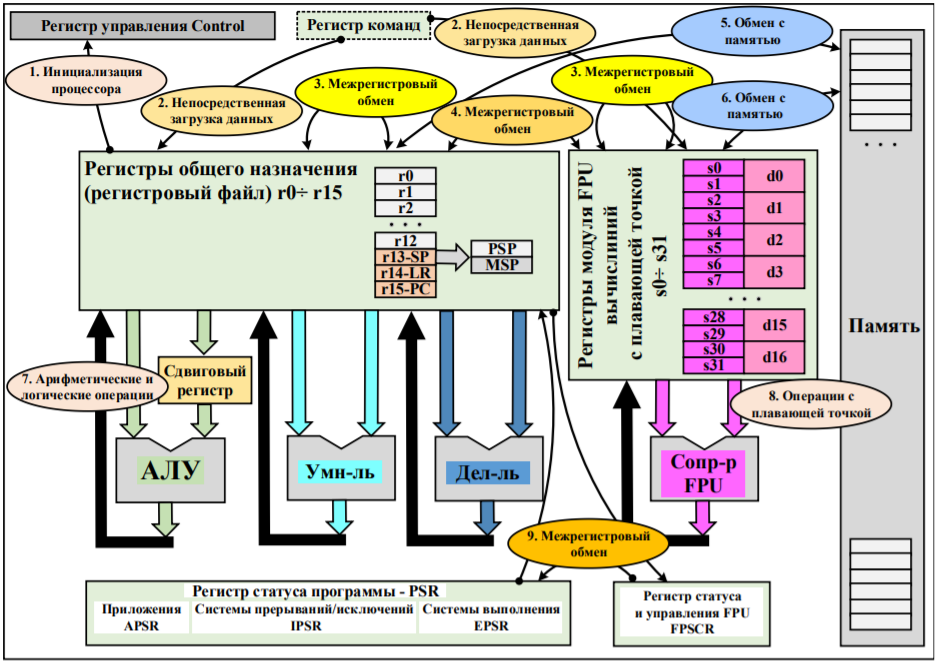
\includegraphics[scale=0.75]{Program_model_ARM.png}
    \caption{Программная модель микроконтроллера ARM Cortex M~\cite{Program_model_ARM}}
    \label{fig:prog_mod_ARM}
\end{figure}

Регистр управления Control --- регистр специального назначения, который позволяет установить нужный режим работы процессора, задать тип доступа к памяти (привилегированный или непривилегированный), разрешить или запретить работу встроенных в процессор устройств, в частности, модуля поддержки вычислений с плавающей точкой (FPU).

Регистр статуса программы (PSR) состоит из трех регистров: регистр статуса программы-приложения (APSR), регистр статуса системы прерываний и исключений (IPSR), регистр статуса системы выполнения команд (EPSR). К каждому из регистров можно обращаться по его персональному имени. Также, по символическому имени можно обращаться к регистру PSR.

Все регистры статуса являются регистрами специального назначения и доступ к ним возможен только с помощью специальных команд обмена данными между регистрами общего назначения ЦП и регистрами специального назначения.

Регистр команд – содержит код операции, подлежащий расшифровке в данный момент.

В памяти программ (ROM) хранится исполняемый код программы, а также могут храниться некоторые данные (константы, таблицы констант).

В памяти данных (RAM) хранятся данные исполняемой программы, кроме того, в ней может храниться код программы. Также, RAM содержит побитово-, побайтово-адресуемую память.

Регистры модуля поддержки вычислений с плавающей точкой (FPU), которые еще называют регистровым окружением сопроцессора FPU, необходимы для хранения операндов, которые используются модулем FPU. Поскольку, FPU может выполнять операции только над операндами, расположенными в его регистрах окружения. 

Имеется 32 регистра s0-s31, предназначенных для хранения данных в формате с плавающей точкой однократной точности. Все регистры 32-разрядные. Каждая пара регистров s0-s31 с точки зрения программиста может рассматриваться как один 64-разрядный регистр. Он может содержать данные в формате с плавающей точкой двойной точности или два слова с плавающей точкой однократной точности. Всего в окружении сопроцессора 16 таких регистров с именами d0-d15.

Регистр статуса и управления модулем поддержки вычислений с плавающей точкой (FPSCR) обеспечивает полный контроль программиста за режимом работы и текущим состоянием модуля FPU. Он позволяет установить нужный для приложения пользователя режим работы, проверить текущее состояние вычислительного процесса по результатам сравнения переменных в формате с плавающей точкой или на предмет возникновения исключительной ситуации (возможной некорректности выполненных вычислений с операндами в формате с плавающей точкой).

В соответствии с этими тремя важнейшими функциями в регистре имеются три группы битовых полей: (r31-r28) --- флаги результатов операций сравнения чисел с  плавающей точкой; (r26-r22) –-- биты управления режимом работы сопроцессора; (r7-r0) --- биты флагов исключительных ситуаций, возникающих при обработке данных.

\subsection{Периферия}

Перифирия микроконтроллеров с архитектурой ARM хорошо развита и включает в себя порты ввода-вывода, система прерываний, АЦП, таймеры общего назначения, сторожевой таймер, расширенный таймер, часы реального времени, последовательный периферийный трехпроводный интерфейс SPI, модуль I2C, модуль УСАПП и др~\cite{ARM-M3}.

Порты ввода-вывода (GPIO) микроконтроллеров ARM являются двунаправленными и, в зависимости от модели микроконтроллера, могут содержать до 80 линий и больше. При этом, для каждого порта имеется 2 конфигурационных регистра, благодаря которым можно настроить порты, узнать в каком направлении работает линия: на ввод или на вывод, а также защитить конфигурационные параметры с помощью регистра блокировки.

Прерывания в микроконтроллерах ARM делится на внешние и внутренние.

Внутренние прерывания осуществляются при помощи контроллера вложенных векторизованных прерываний (КВВП). У любого Cortex-микроконтроллера будет присутствовать одна и та же структура прерываний, независимо от его производителя. Таким образом, прикладной код и операционные системы можно легко портировать с одного МК на любой другой.

КВВП поддерживаются вложенные прерывания и, зачастую, в МК используется несколько уровней приоритетов. Структура прерываний КВВП разработана с учетом программирования полностью на C и исключает потребность в написании каких-либо ассемблерных макросов или специальных, несовместимых с ANSI, директив. О работе системы прерываний подробнее написано в главе об AVR-микроконтроллерах.

Блок внешних прерываний имеет линии прерывания, которые связываются с векторами прерываний посредством КВВП. Блок внешних прерываний играет важную роль для управления энергопотреблением микроконтроллера. Данный блок является асинхронным и, поэтому, может использоваться для возобновления работы микроконтроллера, находящегося в режиме STOP, когда оба основных генератора отключены.

Аналого-цифровой преобразователь необходим для получения числового значения напряжения, поданного на его вход. В зависимости от модели микроконтроллера в него может быть встроено от 1 до 3 аналого-цифровых преобразователей. Вся настройка АЦП выполняется через регистры управления и статуса. Режим работы АЦП задается через два регистра управления.

АЦП питаются отдельным напряжением, которое в зависимости от типа корпуса может находиться в пределах 2.4-3.6 В. Источник опорного напряжения АЦП соединен либо внутренне с напряжением питания АЦП, либо со специальными внешними выводами. АЦП характеризуется 12-битной разрешающей способностью и частотой преобразования 1МГц. У него имеется до 18 мультиплексированных каналов, 16 из которых можно использовать для измерения внешних сигналов. Оставшиеся два канала связаны со встроенным датчиком температуры и внутренним источником опорного напряжения.

Также АЦП поддерживают функцию оконного компаратора, которая заключается в генерации прерывания при выходе результата преобразования за пределы заданных пользователем нижней и верхней границ.

Все блоки таймеров общего назначения выполнены на основе 16-битного перезагружаемого счетчика, который синхронизируется с выхода 16-битного предделителя. Перезагружаемое значение хранится в отдельном регистре. Счет может быть прямой, обратный или двунаправленный. Вход синхронизации счетчика можно связать с одним из восьми различных источников. В их число входят: специальный сигнал синхронизации, производный от сигнала главной системной синхронизации; выходной сигнал синхронизации одного из других таймеров или внешний сигнал синхронизации, связанный с выводами захвата/сравнения.

Каждый из таймеров может генерировать прерывания и поддерживает прямой доступ к памяти (DMA).

Расширенный таймер архитектурно похож на таймеры общего назначения с той разницей, что он дополнен рядом аппаратных узлов, предназначенных для управления электродвигателем.

В каждом из трех каналов этого таймера предусмотрены два противофазных выхода. Таким образом, он представляет собой 6-канальный ШИМ-блок.

Входящие в МК часы реального времени (ЧРВ) представляют собой 32-битный счетчик, оптимизированный под счет секунд при синхронизации частотой 32.768 кГц. Во время настройки системы синхронизации, в качестве источника синхронизации часов реального времени можно выбрать внутренний низкочастотный генератор, внешний низкочастотный генератор или внешний высокочастотный генератор. После выбора источник синхронизации соединяется с часами реального времени через делитель частоты с фиксированным коэффициентом деления. Для организации точного счета секунд далее может быть задействован еще один предделитель ЧРВ.

Сброс МК может быть выполнен встроенными сторожевыми таймерами, программно через контроллер вложенных векторизованных прерываний, встроенными схемами сброса при подаче/отключении и снижении ниже допустимого уровня напряжения питания.

В МК на базе архитектуры ARM, зачастую, входят два типа отдельных сторожевых таймера: независимый и оконный. Независимый сторожевой таймер полностью отделен от основной системы МК. Он расположен в домене с резервированием питания и синхронизируется встроенным низкочастотным генератором (LSI). Оконный сторожевой таймер является частью основной системы МК и связан с сигналом синхронизации первой шины устройства ввода-вывода. Оба сторожевых таймера поддерживают возможность раздельного включения/отключения и могут использоваться одновременно.

Для организации быстродействующей связи с интегральными схемами у микроконтроллеров ARM имеется модуль SPI, предназначенный для полнодуплексной передачи данных. Подробнее про этот интерфейс написано в главе про микроконтроллеры AVR.

Для связи с интегральными схемами у МК имеется еще один специальный интерфейс --- I2C. Интерфейс I2C может работать в ведущем или подчиненном режиме и поддерживает возможность арбитра шины, что необходимо в мультимастерных системах.

Модуль I2C использует 7- и 10-битные режимы адресации. Модуль полностью реализует протокол передачи данных по шине и требует для управления только необходимой протоколу передачи информации. Модуль I2C может генерировать два прерывания: одно при обнаружении ошибок и другое для управления адресом связи и передаваемыми данными. Кроме того, блок DMA предоставляет два канала, которые можно использовать для чтения из буфера передачи и записи данных в этот буфер. Таким образом, сразу после задания адреса и подлежащих передаче данных можно начать двунаправленную передачу данных полностью под аппаратным управлением.

Модуль I2C является аналогом интерфейса TWI в МК AVR.

Несмотря на то, что порты последовательной связи уже практически не используются в ПК, они все еще остаются популярными во многих встраиваемых применениях для организации простого интерфейса последовательной связи. В ARM-микроконтроллерах интегрируется от одного до нескольких модулей УСАПП, каждый из которых поддерживает несколько расширенных режимов работы, позволяющие использовать МК в современных коммуникационных применениях.

Каждый УСАПП имеет собственный генератор скорости связи с возможностями дробного деления частоты. В отличие от обычных делителей частоты, такой генератор позволяет получить стандартные скорости связи при любой частоте синхронизации шины. Также как и остальные модули последовательных интерфейсов, каждый модуль УСАПП оснащен двумя каналами прямого доступа к памяти для двунаправленной связи с буфером данных. В конфигурации УАПП, модуль УСАПП может работать в нескольких режимах работы. УСАПП имеет возможность работы с однопроводной полудуплексной линией. Для связи с модемами, а также для аппаратного управления передачей потока данных, у каждого УСАПП предусмотрены дополнительные линии управления CTS и RTS.

Помимо работы в роли высокоскоростного интерфейса, каждый УСАПП может быть переведен в режим синхронной связи. Его можно использовать для связи с внешними устройствами ввода-вывода, оснащенными SPI-совместимым интерфейсом, по 3-проводной линии. Работая в данном режиме, УСАПП работает в роли ведущего шины SPI и поддерживает возможность программирования полярности и фазы синхронизации. Благодаря этому, возможна связь с практически любой подчиненной SPI ИС.

Как и микроконтроллеры AVR, ARM-микроконтроллеры поддерживают такие модули как CAN, USB, LCD. Подробнее о них написано в главе про AVR~\cite{ARM-M3}.

\subsection{Питание}

Для работы микроконтроллеров ARM их необходимо питать одним напряжением в диапазоне от 1.2 до 5.5 В. В домене с отдельным питанием расположены часы реального времени и небольшое число регистров, что позволяет организовать их резервное питание и обеспечить работоспособность даже при нахождении МК в режиме полного отключения (deep power down)~\cite{ARM-M3}.

ARM микроконтроллер может работать в одном из следующих режимов~\cite{Power_ARM}:

\begin{itemize}
    \item Run --- активный режим работы. В данном режиме процессорное ядро активно и может работать с максимальным быстродействием. Память и периферия доступны без каких-либо ограничений, программный код выполняется из SRAM или Flash;
    
    \item Low-Power Run --- малопотребляющий активный режим с отключенным основным регулятором (MR) и питанием домена VCORE от малопотребляющего регулятора (LPR). В данном режиме ограничена максимальная частота системы и возможность записи и стирания Flash, однако программный код по-прежнему может выполняться из SRAM или Flash;
    
    \item Sleep --- режим работы, при котором тактирование ядра отключено, периферия (в том числе системная), а также память находятся в активном состоянии. Выход из режима и пробуждение процессора происходят при возникновении определенных событий или прерываний;
    
    \item Low-Power Sleep --- режим, сравнимый по принципу работы со Sleep, но для питания домена VCORE используется регулятор (LPR), а основной регулятор (MR) отключается для снижения энергопотребления;
    
    \item Stop 0 --- при переходе в этот режим содержимое памяти SRAM и всех регистров фиксируется. Все сигналы тактирования в домене VCORE останавливаются. Генераторы отключены. Однако некоторые периферийные блоки могут активировать HSI16 для своих потребностей. Для тактирования используются LSI и LSE. В режиме Stop 0 используется регулятор MR, который обеспечивает минимальную задержку при пробуждении ядра, но при этом увеличивает энергопотребление;
    
    \item Stop 1 – режим, аналогичный Stop 0, но для питания домена VCORE используется регулятор LPR, а регулятор MR отключается с целью снижения потребления, однако такой подход увеличивает время пробуждения контроллера;
    
    \item Standby With SRAM2 --- режим ожидания с памятью SRAM2. При работе в данном режиме питание домена VCORE отключено, однако содержимое SRAM2 может быть сохранено. Питание SRAM2 осуществляется от регулятора LPR. Все сигналы тактирования в домене VCORE, а также генераторы --- остановлены. Для тактирования могут использоваться LSI и LSE. Выход из режима может происходить при сбросе, некоторых событиях, а также при подаче сигнала на соответствующие выводы микроконтроллера;
    
    \item Standby Without SRAM2 --- аналогичен предыдущему режиму, однако содержимое SRAM2 не сохраняется. Регулятор LPR отключен;
    
    \item Shutdown --- режим, при котором питание домена VCORE отключено. Все сигналы тактирования в домене VCORE, а также генераторы --- остановлены. Для тактирования доступен только LSE. В данном режиме также отключаются блоки мониторинга напряжения.
\end{itemize}

\chapter{Программное и аппаратное обеспечение для AVR и ARM микроконтроллеров}
\section{Arduino}

Arduino --- торговая марка аппаратно-программных средств для построения и прототипирования простых систем, моделей и экспериментов в области электроники, автоматики, автоматизации процессов и робототехники~\cite{wikiRUArduino}.

\subsection{Программная часть}

Программная часть состоит из бесплатной программной оболочки (IDE) для написания программ, их компиляции и программирования аппаратуры. Аппаратная часть представляет собой набор смонтированных печатных плат, продающихся как официальным производителем, так и сторонними производителями. Полностью открытая архитектура системы позволяет свободно копировать или дополнять линейку продукции Arduino (рис. 2.1).

\begin{figure}[H]
    \centering
    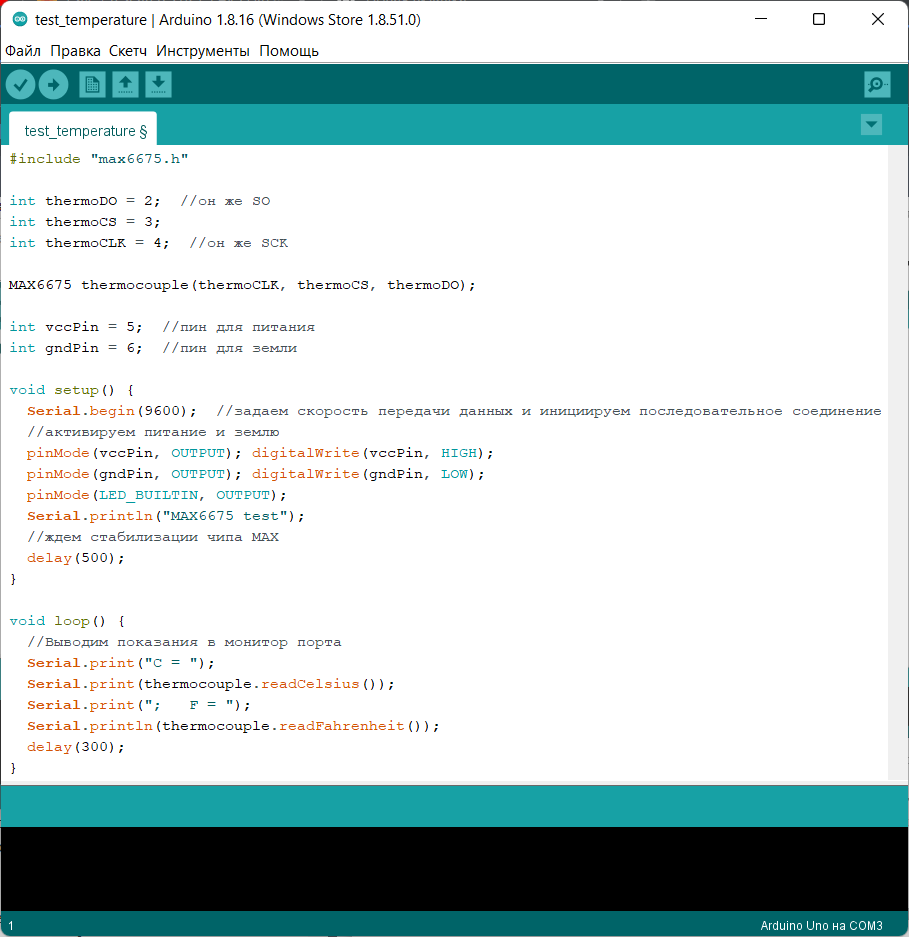
\includegraphics[scale=0.6]{Arduino_IDE.png}
    \caption{Arduino IDE с примером простой программы}
    \label{fig:ide}
\end{figure}

Используется как для создания автономных объектов, так и подключения к программному обеспечению через проводные и беспроводные интерфейсы. Подходит для начинающих пользователей с минимальным входным порогом знаний в области разработки электроники и программирования.

Программирование ведется целиком через собственную бесплатную программную оболочку Arduino IDE. В этой оболочке имеется текстовый редактор, менеджер проектов, препроцессор, компилятор и инструменты для загрузки программы в микроконтроллер. Оболочка написана на Java на основе проекта Processing, работает под Windows, Mac OS X и Linux. Используется комплект библиотек Arduino.

\subsection{Язык программирования}

Язык программирования Arduino называется Arduino C и представляет собой язык C++ с фреймворком Wiring, он имеет некоторые отличия по части написания кода, который компилируется и собирается с помощью avr-gcc, с особенностями, облегчающими написание работающей программы — имеется набор библиотек, включающий в себя функции и объекты. При компиляции программы IDE создает временный файл с расширением *.cpp.

Программы, написанные программистом Arduino, называются скетчи и сохраняются в файлах с расширением *.ino. Эти файлы перед компиляцией обрабатываются препроцессором Arduino. Также существует возможность создавать и подключать к проекту стандартные файлы C++.

Программист должен написать две обязательные для Arduino функции setup() и loop(). Первая вызывается однократно при старте, вторая выполняется в бесконечном цикле.

В текст своей программы (скетча) программист не обязан вставлять заголовочные файлы используемых стандартных библиотек. Эти заголовочные файлы добавит препроцессор Arduino в соответствии с конфигурацией проекта. Однако пользовательские библиотеки нужно указывать.

Менеджер проекта Arduino IDE имеет нестандартный механизм добавления библиотек. Библиотеки в виде исходных текстов на стандартном C++ добавляются в специальную папку в рабочем каталоге IDE. При этом название библиотеки добавляется в список библиотек в меню IDE. Программист отмечает нужные библиотеки, и они вносятся в список компиляции.

Arduino IDE не предлагает никаких настроек компилятора и минимизирует другие настройки, что упрощает начало работы для новичков и уменьшает риск возникновения проблем; но присутствуют директивы препроцессора, такие как \#define, \#include и много других.

Закачка программы в микроконтроллер Arduino происходит через предварительно запрограммированный специальный загрузчик (все микроконтроллеры от Arduino продаются с этим загрузчиком). Загрузчик создан на основе Atmel AVR Application Note AN109. Загрузчик может работать через интерфейсы RS-232, USB или Ethernet в зависимости от состава периферии конкретной процессорной платы. В некоторых вариантах, таких как Arduino Mini или неофициальной Boarduino, для программирования требуется отдельный переходник.

Пользователь может самостоятельно запрограммировать загрузчик в чистый микроконтроллер. Для этого в IDE интегрирована поддержка программатора на основе проекта AVRDude. Поддерживается несколько типов популярных дешёвых программаторов.

\subsection{Аппаратная часть}

Под торговой маркой Arduino выпускается несколько плат с микроконтроллером и платы расширения. Большинство плат с микроконтроллером снабжено минимально необходимым набором обвязки для нормальной работы микроконтроллера (стабилизатор питания, кварцевый резонатор, цепочки сброса и т. п.).

В концепцию Arduino не входит корпусного или монтажного конструктива. Разработчик выбирает метод установки и механической защиты плат самостоятельно либо с помощью сторонних компаний. Сторонними производителями также выпускаются наборы робототехнической электромеханики, ориентированной на работу совместно с платами Arduino. Независимыми производителями также выпускается большое количество всевозможных датчиков и исполнительных устройств, в той или иной степени совместимых с Arduino (рис. 2.2)~\cite{UNO}.

\begin{figure}[!ht]
    \centering
    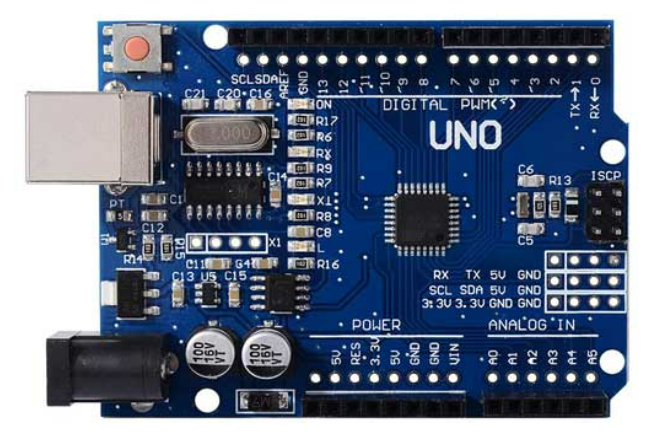
\includegraphics{Arduino_Uno.png}
    \caption{Отладочная плата Arduino Uno}
    \label{fig:uno}
\end{figure}

\subsection{Классический конструктив}

Классические Arduino и Arduino-совместимые платы спроектированы для монтажа в стопки через штыревые разъёмы. Таким образом базовую микропроцессорную плату дополняют необходимой периферией и внешними подключениями.

Существуют платы Uno, Pro, Leonardo, Mega 2560, Due и платы, например Zero, с расширенным набором штыревых разъёмов для них. Платы расширения стандартной длины могут устанавливаться и в расширенные процессорные платы~\cite{Arduino}.

\subsection{Миниатюрный конструктив}

\begin{center}
    \textbf{Arduino}
\end{center}

Выпускаются отдельные платы уменьшенных габаритов — Nano, Nano Every и Micro — в габарите DIP-корпусов микросхем. Они предназначены для установки в макетные платы. Плат расширения для них нет.

Позже была выпущена линейка Arduino MKR в похожем конструктиве. К ним есть небольшой набор плат расширения периферии.

\begin{center}
    \textbf{Сторонние проекты}
\end{center}

Помимо стандартных конструктивов Arduino, сторонние разработчики создали множество миниатюрных клонов, сохранив только архитектурную и программную совместимость. Среди этих клонов выделяется линейка продуктов Microduino. Линейка содержит полноценный набор конструктивно совместимых процессорных модулей, модулей связи, датчиков и исполнительных устройств, практически не уступая ассортименту классических модулей Arduino. Как и Arduino, сборка плат производится в стопки. Линейка оформлена в двух оригинальных конструктивах:

\begin{itemize}
    \item Бескорпусной, с соединениями на миниатюрных цанговых штыревых линейках.

    \item В стиле конструкторов Лего с электрическими соединениями на подпружиненных контактах и механической фиксацией, совместимой с конструкторами Лего.
\end{itemize}

\subsection{Микроконтроллер}

Микроконтроллеры для Arduino отличаются наличием предварительно прошитого в них загрузчика. С помощью этого загрузчика пользователь загружает свою программу в микроконтроллер без использования традиционных отдельных аппаратных программаторов. Загрузчик соединяется с компьютером через интерфейс USB (если он есть на плате) или с помощью отдельного переходника UART-USB. Поддержка загрузчика встроена в Arduino IDE.

На случай затирания загрузчика или покупки микроконтроллера без загрузчика разработчики предоставляют возможность прошить загрузчик в микроконтроллер самостоятельно. Для этого в Arduino IDE встроена поддержка нескольких популярных дешевых программаторов, а большинство плат Arduino имеет штыревой разъём для внутрисхемного программирования (ICSP для AVR, JTAG или SWD для ARM).

В Arduino IDE встроена возможность создания своих программно-аппаратных платформ. Этой возможностью пользуются сторонние компании, которые добавляют в Arduino IDE свои наборы плат и компиляторов-загрузчиков к ним.

\begin{center}
    \textbf{AVR}
\end{center}

В классической линейке устройств Arduino в основном применяются микроконтроллеры Atmel AVR. Следующие микроконтроллеры можно встретить на указанных распространённых платах:~\cite{Blum}

\begin{itemize}
    \item ATmega2560 (16 МГц, 256 Kb Flash, 8 Kb RAM, 54 порта, из них до 15 с ШИМ и 16 АЦП). Платы Mega.

    \item ATmega32U4 (16 МГц, 32 Kb Flash, 2,5 Kb RAM, 20 портов, из них до 7 с ШИМ и 12 АЦП). Платы Leonardo, Micro, Yun.

    \item ATmega328 (16 МГц, 32 Kb Flash, 2 Kb RAM, 14 портов, из них до 6 с ШИМ и 8 АЦП). Платы UnoR3, Mini, NanoR2, Pro, Pro mini, различные варианты плат uno и nano, такие как Wifi Uno и nano + nrf42l01

    \item ATtiny85 (20 Мгц, 8 Kb Flash, 512 b RAM, 6 портов, из них 4 ШИМ и 4 аналоговых). Платы Digispark, также часто применяются вне плат.

    \item ATmega168 (16 Мгц, 16 Kb Flash, 1 Kb RAM, порты и распиновка аналогично ATmega328) Платы Uno R1, Uno R2, Pro mini, NanoR1.
\end{itemize}

В некоторых платах состав доступных портов и частота тактирования могут отличаться.

\begin{center}
    \textbf{ARM}
\end{center}

Постепенно в линейке плат стали появляться процессоры ARM. Первоначально это был AT91SAM3X8E на плате классического конструктива (Due). Позже появилась линейка плат Arduino MKR в конструктиве DIP, оснащенная контроллером SAMD21 (Cortex-M0, 48 MHz, 256 Kb Flash, 32 Kb RAM).

С 2020 года в таком же конструктиве MKR появились модули Portenta с ARM Cortex-M7 (STM32H747 @ 480 МГц).

\begin{center}
    \textbf{ESP8266}
\end{center}

Сторонние разработчики портировали в Arduino поддержку популярного Wi-Fi микроконтроллера ESP8266 и его клона ESP12. Компилировать и загружать прошивку для ESP8266 со своими скетчами и поддержкой Wi-Fi можно прямо из Arduino IDE, получая одноплатную схему с поддержкой сети Wi-Fi.

\begin{center}
    \textbf{Intel x86}
\end{center}

В рамках сотрудничества со сторонними производителями в Arduino IDE была включена поддержка некоторых аппаратных средств Intel x86. Intel Galileo, Intel Edison и Arduino 101 --- Arduino-совместимые платы на Intel x86 архитектуре. Платы механически и электрически совместимы с периферийными платами Arduino. Платы функционируют под собственной ОС Linux, поверх которой работает приложение, позволяющее загружать и исполнять скетчи Arduino.

\subsection{Периферия}

Порты ввода-вывода микроконтроллеров оформлены в виде штыревых линеек. Никакой буферизации, защиты, конвертации уровней, как правило, нет. Микроконтроллеры питаются от 5 В или 3,3 В в зависимости от модели платы. Соответственно, порты имеют такой же размах допустимых входных и выходных напряжений. Программисту доступны некоторые специальные возможности портов ввода-вывода микроконтроллеров, например широтно-импульсная модуляция (ШИМ), аналогово-цифровой преобразователь (АЦП), интерфейсы UART, SPI, I2C. Количество и возможности портов ввода-вывода определяются конкретным вариантом микропроцессорной платы.

Помимо портов, на платах микроконтроллеров иногда устанавливается периферия в виде интерфейсов USB или Ethernet. Опциональный набор внешней периферии на модулях расширения включает в себя:

\begin{itemize}
    \item USB Device (чаще всего как виртуальный COM порт, имеются также версии с эмуляцией USB HID Class клавиатур и мышек).

    \item Проводной и беспроводной Ethernet как на основной плате, так и на платах расширения.

    \item Модуль GSM и другие беспроводные интерфейсы.

    \item USB Host.

    \item SD card.

    \item Модуль управления низковольтным мотором.

    \item Графический ЖКИ-индикатор.

    \item Модуль с макетным полем.
\end{itemize}

Сторонние производители выпускают широкий выбор датчиков и исполнительных устройств, подключаемых к Arduino. Например, гироскопы, компасы, манометры, гигрометры, термометры, релейные модули, индикаторы, клавиатуры и т. п.

\begin{center}
    \textbf{FPGA}
\end{center}

Существуют совместимые с Arduino процессорные платы, на которых в качестве периферийного устройства установлена микросхема программируемой логики (FPGA). Например, сама компания Arduino выпускает плату Arduino MKR Vidor 4000, на которой, помимо процессора, установлена ПЛИС Intel Cyclone. Программист в среде Arduino может загружать в FPGA предустановленные функции, например, работу с изображениями, звуком, дополнительные порты UART, SPI, ШИМ и т.д. Однако, свободное программирование FPGA из среды Arduino не предусмотрено, для этого необходимо использовать среду разработки производителя FPGA --- Intel Quartus.

Также существует проект Papilio, в котором развивается совместимая с Arduino линейка плат с программируемой логикой Xilinx в качестве периферии. Помимо готовых решений для использования FPGA в качестве периферии, проект предлагает интеграцию среды программирования Arduino и среды программирования FPGA Xilinx ISE schematic editor. Пользователь может редактировать FPGA аналогично рисованию электрических схем.

\section{Другое популярное программное обеспечение для AVR и ARM микроконтроллеров}

Помимо Arduino IDE большой популярностью пользуются следующие решения:~\cite{MK}~\cite{MK_2}

\begin{enumerate}
    \item Atmel Studio --- интегрированная среда разработки (IDE) от компании Atmel для разработки приложений под микроконтроллеры ARM Cortex-M и AVR. Распространяется бесплатно.
    
    \item AVRDUDE --- интерфейс программы консольный, предназначена, чтобы изменять и записывать данные в памяти устройств c AVR архитектурой. В программе применяется технология внутрисхемного программирования. Распространение свободное.
    
    \item WinAVR --- мощная среда разработки с открытым исходным кодом, созданная с целью написания программ для микроконтроллеров серии AVR от компании Atmel. Распространяется свободно и бесплатно.
    
    \item VM LAB --- комплекс утилит для создания и настройки кода программы, на ряду с этим создает модель работы устройства с контроллерами AVR серии. Распространяется свободно.
    
    \item MPLAB --- единая бесплатная интегрированная среда разработки для контроллеров производства Microchip.
    
    \item CooCoxCoIDE --- работает с устройствами в чью архитектуру заложен ARM, как программная среда с высокой степенью интеграции.
\end{enumerate}

Также существует еще ряд программ: BascomAVR, CodeVisionAVR, WinPic800, PICPgm, Keil uVision, IAR Embedded Workbench, Flow Сode, Atollic TrueSTUDIOб Sourcery CodeBench и др. Но такие решения в основном предоставляются на платной основе или с урезанным функционалом для бесплатных версий.

\chapter*{Заключение}
\addcontentsline{toc}{chapter}{Заключение}

В результате научно-исследовательской работы были выполнены следующие задачи:

\begin{enumerate}
    \item Осуществлено знакомство с архитектурой микроконтроллеров AVR и ARM на примере представителя каждого семейства.
    
    \item Осуществлено знакомство с наборами команд для микроконтроллеров семейств AVR и ARM.
    
    \item Изучены некоторые аппаратные и программные средства для разработки под AVR и ARM микроконтроллеры, подходящие для дальнейшего обучения и разработки на начальном уровне.
\end{enumerate}

В дальнейшем предполагается применение полученных знаний для разработки собственного программного продукта на выбранной аппаратно-программной базе.

\newpage
\addcontentsline{toc}{chapter}{Список использованной литературы}
\printbibliography[title={Список использованной литературы}]

\end{document}
